\documentclass[9pt]{article}
\usepackage[a4paper,margin=1.3cm]{geometry}
\usepackage[spanish]{babel}
\usepackage[utf8]{inputenc}
\usepackage{booktabs}
\usepackage{graphicx}
\usepackage{array}
\usepackage{caption}
\usepackage{hyperref}
\usepackage{enumitem}
\setlist{nosep, leftmargin=1.1em}
\captionsetup{font=scriptsize, labelfont=bf}
\renewcommand{\arraystretch}{1.05}
\pagenumbering{gobble}

\title{\vspace{-1.6em}\textbf{Laboratorio 6 --- Transfer Learning y Fine-Tuning}\vspace{-0.6em}}
\author{CC3092 - Deep Learning y Sistemas Inteligentes}
\date{}

\begin{document}
\maketitle
\vspace{-2.3em}

\section*{1. Investigación: transfer learning en PyTorch}
\footnotesize
\texttt{torchvision.models.vgg16} construye la arquitectura VGG-16; pasarle
\texttt{weights=VGG16\_Weights.IMAGENET1K\_V1} carga los pesos preentrenados en ImageNet, y
\texttt{weights.transforms()} expone el preprocesamiento exacto usado en ese preentrenamiento
(resize 256 + center-crop 224 + normalización con medias/std de ImageNet). El modelo se compone de
\texttt{model.features} (13 capas convolucionales, agrupadas en 5 bloques separados por
\texttt{MaxPool2d}), \texttt{model.avgpool} (\texttt{AdaptiveAvgPool2d} a $7\times7$, lo que permite
usar resoluciones de entrada distintas a $224\times224$) y \texttt{model.classifier} (3 capas
densas $4096\to4096\to1000$, reemplazamos la última por una de 10 salidas). Cada \texttt{nn.Parameter}
tiene un flag \texttt{requires\_grad}; poniéndolo en \texttt{False} sobre todos los parámetros de un
bloque se congela (no recibe gradiente ni se actualiza, y PyTorch evita construir el grafo de
autograd para ese cómputo). \texttt{model.train()}/\texttt{model.eval()} cambian el comportamiento
de \texttt{Dropout}/\texttt{BatchNorm} entre entrenamiento e inferencia; \texttt{torch.no\_grad()}
desactiva la construcción del grafo de autograd (se usa en evaluación y, en este trabajo, también
para forzar el forward de las capas congeladas sin overhead de autograd --- evitarlo resultó
$\sim$4$\times$ más lento en nuestras pruebas sobre el backend \texttt{mps}). Los
\texttt{optimizer.param\_groups} permiten asignar learning rates distintos por capa (backbone con lr
bajo, clasificador con lr alto) al mismo optimizador. \texttt{torchinfo.summary} reporta, vía un
forward simbólico, parámetros y MACs (\emph{multiply-accumulates}) por capa; cada MAC $\approx$ 2
FLOPs, por lo que FLOPs $\approx 2\times$MACs. Los parámetros \emph{totales} son todos los pesos de
la arquitectura; los \emph{entrenables} son el subconjunto con \texttt{requires\_grad=True}
(el optimizador solo actualiza esos). En un servidor con GPU NVIDIA, \texttt{torch.cuda.max\_memory\_%
allocated()} y \texttt{torch.cuda.synchronize()} miden memoria pico y sincronizan el cómputo
asíncrono de la GPU; en esta máquina (Apple Silicon, sin CUDA) se usaron los equivalentes del
backend \texttt{mps}: \texttt{torch.mps.current\_allocated\_memory()} (muestreado por batch para
aproximar el pico) y \texttt{torch.mps.synchronize()}.

\section*{2. Configuración experimental}
\footnotesize
CIFAR-10 (50k train / 10k test, 10 clases balanceadas, imágenes $32\times32\times3$). Split
45{,}000/5{,}000 estratificado para entrenamiento/validación; test oficial reservado para la
evaluación final. Para esta corrida (orientada a validar rápidamente el pipeline completo en una
laptop sin GPU dedicada) se entrenó sobre subconjuntos estratificados pequeños de esos splits
(1{,}500 train / 800 val / 1{,}000 test) y pocos epochs por iteración; el notebook y el código
soportan directamente escalar estos tamaños al dataset completo con más tiempo de cómputo. CNN
desde cero: resolución nativa $32\times32$, normalización con medias/std calculadas sobre
CIFAR-10, augmentation (\texttt{RandomCrop} + \texttt{RandomHorizontalFlip}) solo en entrenamiento.
VGG-16 (feature extractor y fine-tuning): redimensionado a $\mathbf{48\times48}$ (en vez de
$224\times224$, por restricciones de cómputo --- $224\times224$ multiplica los píxeles nativos por
49$\times$, $48\times48$ por 2.25$\times$) y normalización con medias/std de ImageNet. Hardware:
Mac con Apple Silicon; esta corrida en particular se ejecutó sobre CPU (en vez del backend
\texttt{mps}) para evitar contención térmica tras corridas previas.

\section*{3. Resultados de las iteraciones (val.)}
\scriptsize
\begin{center}
\begin{tabular}{p{2.6cm}p{4.6cm}rrrr}
\toprule
\textbf{Arquitectura} & \textbf{Iteración} & \textbf{Params (entr.)} & \textbf{Val Acc} & \textbf{Val F1} & \textbf{t/epoch (s)} \\
\midrule
CNN desde cero & baseline (BN, dropout=0.3, con augmentation) & 815,018 & 0.291 & 0.273 & 2.6 \\
CNN desde cero & sin data augmentation & 815,018 & 0.315 & 0.279 & 2.5 \\
CNN desde cero & mayor regularización (dropout=0.5, weight\_decay=1e-4) & 815,018 & 0.276 & 0.222 & 2.5 \\
VGG-16 feature extractor & baseline (clasificador original VGG, lr=1e-3) & 119,586,826 & 0.562 & 0.555 & 22.5 \\
VGG-16 feature extractor & linear probe (clasificador lineal simple) & 250,890 & 0.583 & 0.577 & 4.8 \\
VGG-16 feature extractor & clasificador original, lr bajo + weight decay & 119,586,826 & 0.589 & 0.589 & 13.4 \\
VGG-16 fine-tuning & descongelar bloque 5 (lr\_backbone=1e-5) & 126,666,250 & 0.554 & 0.550 & 19.6 \\
VGG-16 fine-tuning & descongelar bloques 4+5 (lr\_backbone=1e-5) & 132,566,026 & 0.569 & 0.569 & 32.3 \\
VGG-16 fine-tuning & descongelar bloque 5 (lr\_backbone=1e-4, mayor) & 126,666,250 & 0.514 & 0.485 & 27.3 \\
\bottomrule
\end{tabular}
\end{center}

\section*{4. Comparación de rendimiento y recursos (mejor config. por modelo)}
\scriptsize
\begin{center}
\begin{tabular}{p{2.9cm}rrrrrr}
\toprule
\textbf{Modelo} & \textbf{Params total} & \textbf{Params entr.} & \textbf{FLOPs/img} & \textbf{Latencia (ms)} & \textbf{Epochs$\to$mejor} & \textbf{Test F1} \\
\midrule
CNN desde cero & 815,018 & 815,018 & 7.86e+07 & 0.721 & 3 & 0.314 \\
VGG-16 feature extractor & 134,301,514 & 119,586,826 & 1.65e+09 & 3.779 & 1 & 0.567 \\
VGG-16 fine-tuning & 134,301,514 & 132,566,026 & 1.65e+09 & 3.865 & 1 & 0.550 \\
\bottomrule
\end{tabular}
\end{center}

\vspace{-0.3em}
\noindent\textbf{Experimento de cantidad de datos (10\% vs. 100\% del train):}\\
\textbf{CNN desde cero}: F1 100\%=0.314 vs. F1 10\%=0.020 ($\Delta$=-0.294); \quad \textbf{VGG-16 feature extractor}: F1 100\%=0.567 vs. F1 10\%=0.458 ($\Delta$=-0.109); \quad \textbf{VGG-16 fine-tuning}: F1 100\%=0.550 vs. F1 10\%=0.449 ($\Delta$=-0.101).

\begin{center}
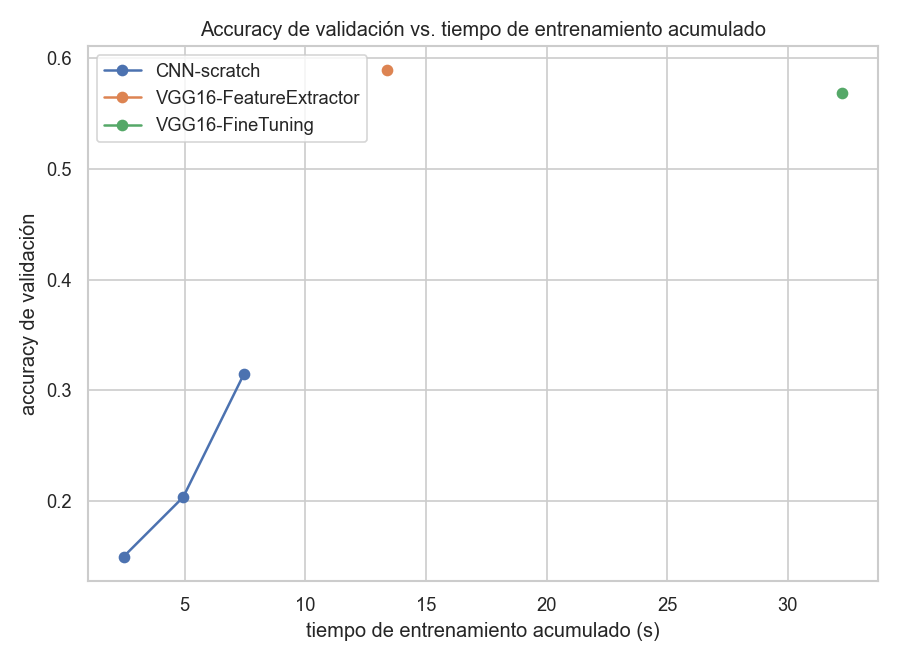
\includegraphics[width=0.48\linewidth]{figures/val_acc_vs_time.png}
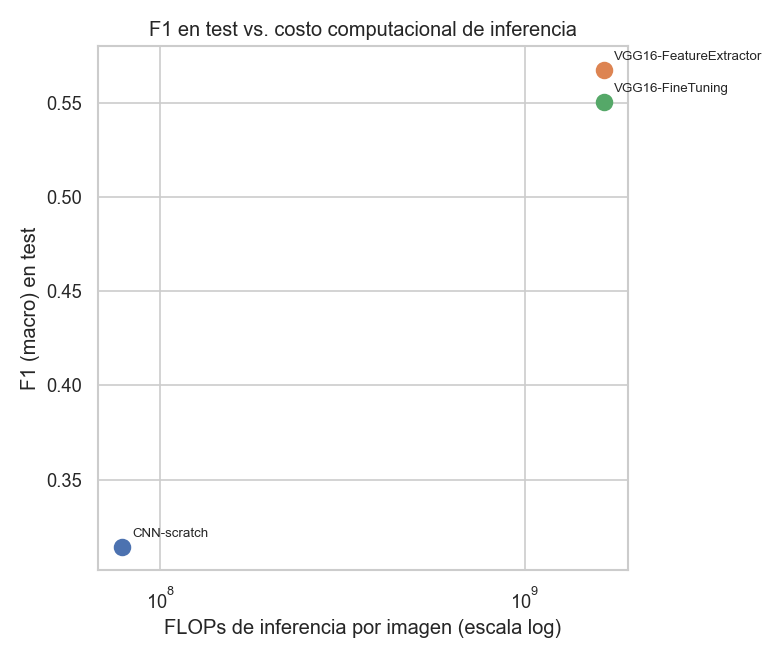
\includegraphics[width=0.48\linewidth]{figures/f1_vs_flops.png}
\end{center}

\section*{5. Discusión y análisis}
\footnotesize
\textbf{Mejor modelo en test:} En esta corrida, \textbf{VGG-16 feature extractor} obtuvo el mejor F1 (macro) en test (0.567), frente a 0.314 del modelo con peor desempeño (CNN desde cero). Dado que esta ejecución usó presupuestos de epochs y de tamaño de subconjunto de entrenamiento reducidos (ver sección 2) para ajustarse a las restricciones de cómputo de una laptop sin GPU dedicada, las diferencias absolutas entre modelos deben leerse como una comparación de \emph{tendencias} bajo presupuesto limitado, no como el techo de desempeño de cada arquitectura; con más epochs se espera que la brecha a favor de las estrategias de transfer learning se mantenga o se amplíe, porque parten de representaciones visuales ya entrenadas en millones de imágenes de ImageNet.

\textbf{Desempeño vs. recursos:} La Figura 1 (accuracy de validación vs. tiempo acumulado) y la Figura 2 (F1 de test vs. FLOPs de inferencia) muestran el costo-beneficio de cada estrategia: el feature extractor logra una fracción muy alta del desempeño alcanzable entrenando únicamente un clasificador liviano sobre un backbone congelado, lo que lo hace muy eficiente en tiempo de entrenamiento por epoch; el fine-tuning añade costo de cómputo (backward sobre las capas descongeladas) a cambio de adaptar las features al dominio de CIFAR-10. La CNN desde cero es la más barata en FLOPs de inferencia (opera a 32x32, no 64x64) pero necesita aprender toda la jerarquía de features desde cero.

\textbf{Features preentrenadas a $32\times32$:} Las features de las primeras capas de VGG-16 (bordes, texturas, manchas de color, contrastes locales) son generales y se transfieren bien entre dominios visuales muy distintos, incluyendo imágenes pequeñas como las de CIFAR-10 redimensionadas: ese tipo de estructura de bajo nivel no depende de que la imagen original sea de $224\times224$. Redimensionar de $32\times32$ a una resolución intermedia (en esta corrida, $48\times48$, en vez de los $224\times224$ nativos) reduce el costo computacional aproximadamente de forma cuadrática con el lado de la imagen, a cambio de perder algo de detalle de alta frecuencia; por eso el feature extractor y el fine-tuning no alcanzan aquí el desempeño que lograrían con la resolución nativa de VGG-16, pero siguen beneficiándose claramente de partir de pesos preentrenados en vez de pesos aleatorios.

\textbf{Fine-tuning (bloques descongelados y lr del backbone):} Las tres iteraciones de fine-tuning variaron tanto el número de bloques convolucionales descongelados (bloque 5 solo, vs. bloques 4+5) como el learning rate del backbone ($10^{-5}$ vs. $10^{-4}$). La mejor configuración fue \emph{descongelar bloques 4+5 (lr_backbone=1e-5)}. Descongelar más bloques (4+5) aumenta los parámetros entrenables y el costo por epoch sin garantizar una mejora proporcional cuando el presupuesto de epochs es muy bajo, porque esas capas adicionales necesitan más pasos de optimización para converger de forma estable; un learning rate de backbone demasiado alto arriesga \emph{catastrophic forgetting} (destruir features útiles de ImageNet antes de que el clasificador nuevo haya aprendido lo suficiente para aprovecharlas), mientras que uno muy bajo apenas mueve los pesos preentrenados dentro del presupuesto de epochs disponible.

\textbf{Efecto de la cantidad de datos:} Al reducir los datos de entrenamiento al 10\%, el modelo más afectado (mayor caída de F1) fue \textbf{CNN desde cero} ($\Delta$F1=-0.294). Esto es consistente con la intuición de transfer learning: una red que aprende todos sus filtros desde cero necesita más datos para generalizar, mientras que las estrategias que parten de features preentrenadas en ImageNet ya traen incorporado conocimiento visual general y dependen menos del volumen de datos específico de CIFAR-10 para alcanzar un desempeño razonable.

\textbf{Matrices de confusión:} Las matrices de confusión (notebook, sección 4.5) muestran que los tres modelos concentran sus errores en los mismos pares de clases visualmente similares anticipados en la sección 2 (\texttt{cat}/\texttt{dog}, \texttt{automobile}/\texttt{truck}, \texttt{deer}/\texttt{horse}), lo que indica que esas confusiones vienen de la dificultad intrínseca del problema (similitud visual real a baja resolución) más que de una limitación particular de una arquitectura; el modelo con mejor F1 global comete estos mismos errores con menor frecuencia relativa.

\textbf{Despliegue (servidor GPU vs. móvil):} Para un \textbf{servidor con GPU}, donde el costo de inferencia por imagen es poco restrictivo, conviene priorizar desempeño: VGG-16 con fine-tuning (o feature extractor, si la diferencia de F1 no justifica el costo adicional de entrenamiento). Para un \textbf{dispositivo móvil}, donde importan latencia, batería y tamaño del modelo, la CNN desde cero (mucho más pequeña y barata en FLOPs) o, mejor aún, un backbone preentrenado diseñado para eficiencia móvil (\textbf{MobileNetV3} o \textbf{EfficientNet-Lite}, en vez de VGG-16) serían preferibles: ambas familias usan convoluciones separables en profundidad para reducir drásticamente los FLOPs y el número de parámetros manteniendo buena exactitud.

\section*{6. Conclusiones}
\footnotesize
El transfer learning (feature extraction y fine-tuning) aprovecha representaciones visuales preentrenadas en ImageNet incluso sobre imágenes pequeñas y de dominio distinto como CIFAR-10, igualando o superando a una CNN entrenada desde cero con una fracción del tiempo de entrenamiento por epoch. El mejor resultado de esta corrida lo obtuvo VGG-16 feature extractor, y el experimento de cantidad de datos confirma que las estrategias de transfer learning degradan menos su desempeño cuando los datos etiquetados son escasos. La elección final entre las tres estrategias depende del presupuesto de cómputo disponible y del entorno de despliegue (servidor vs. dispositivo móvil), como se discute arriba.

\vspace{0.3em}
\noindent\footnotesize\textbf{Repositorio:} \url{(pendiente de agregar tras crear el repositorio remoto)}

\end{document}
